% Please do not change the document class
\documentclass{scrartcl}

% Please do not change these packages
\usepackage[hidelinks]{hyperref}
\usepackage[none]{hyphenat}
\usepackage{setspace}
\doublespace

% You may add additional packages here
\usepackage{amsmath}
\usepackage{graphicx}

% Please include a clear, concise, and descriptive title
\title{CPD Episode 2: Revenge of the Miscommunication}

% Please do not change the subtitle
\subtitle{COMP130 - CPD Report}

% Please put your student number in the author field
\author{1707981}

\begin{document}

\maketitle

\section{Introduction} % 96 words
I aim to create and run a game production company someday, standing in a high creative (yet additionally technical) position. My experience as scrum master has helped me realise the challenges I face in positions of leadership, particularly in the area of motivating an unpaid leaderless team. This is a good challenge--if I can master this, it will create good grounding for creating a team even with low initial monetary motivation.

Here lies the continuation of my constant adaptation to the social world in pursuit of the destruction of my social awkwardness, obliviousness and frequently mistaken decisions.

% SUMMARY: What do I wanna do!
% Lead a game company as a creative director! Be big idea guy who makes magic happen with his programming skillz!

% How am I gonna get there!
% Get better at communicating ideas!
% - Use illustrative techniques!
% - Get better at drawing!
% Get better at programming!
% - Make projects!
% Get better at reaching out!
% - Use more social medias!
% Motivate other people!
% Get better at initiative!
% Be a leader!

\section{Overview of skill areas}
\subsection{Affective - Regulating work stress} % 203 words (Woo!)
During PASS tutoring training, I teamed up with a peer to plan a session for a dissatisfyingly brief time. We planned to follow up on Facebook, but her messages came in 30-minute intervals, and were short--occasionally one-word answers. I was ultimately stressed in anticipation of a session where I didn't know what would happen, or what role I would play.

Most likely I have a fear of the unknown, resulting in a negative effect on my health, yet a positive influence on my work ethic. The stress, however, is unfavourable for myself and peers. Ultimately, broken communication is unavoidable in the career, along with other circumstances wherein I can't predict the outcome.

This issue won't resolve without raw experience. However, stress is broad, and various unrelated things can reduce it. As a reputable fact for most people (and a compelling theory for programmers), exercise is known to improve mood as well as regular breaks. So from the start of next term, I'll walk a lap around campus for half an hour every Sunday morning. This will introduce more energetic and beneficial forms of break times into my routine, and may help me focus and reduce stress.

% Specific: Yes
% Measurable: No--how can I tell if my stress levels are reduced?
% Achievable: Yes
% Relevant: maybe?
% Time-constrained: Yes

\subsection{Interpersonal - Taking initiative and motivating people (SMART)} % 222 words (Boo!)
As scrum master in Team Duo, one of my duties was to arrange the stand-up times, so I tried to determine which times were most likely to attract the most members. First I introduced polls: ``what times are you free?'' and ``do you prefer post-session or pre-session standups?''. At the time, I felt that working around their believed ideals would make them comfortable coming in. But I eventually realised that their ideals aren't necessarily oriented for good productivity, and akin to a game tester, their beliefs did not always reflect their actual actions.

Also, by essentially giving them the decision, I possibly disrupted the dynamics of a scrum master and their team. For this mostly introverted team, I should have taken more initiative: setting consistent times, assessing how they did, and adjusting them based on the results. Perhaps the results don't matter so much as the motivation and enthusiasm, which should take focus.

That requires persuasion and motivational skills, which I would benefit greatly from understanding. One reputable book for this is \textit{``The 7 habits of highly effective people''} by Stephen Covey. I'll read 6 pages per evening, with two days' leeway per week, with the goal of reaching the end of the book by [MONTH HERE] with a greater understanding of motivating a team.

NOTE: needs a start date--the library says the book's there but it clearly isn't where is it!?

% Specific: Yes measurable: Yes Achievable: Yes Relevant: Yes Time-constrained: Yes

\subsection{Dispositional - Self-prioritisation} % 237 words......
Sometimes my assignments took precedence over challenging real-life domestic tasks. I tended to focus on the goals of others. When I had time to work on Handzer or Demiurge, I focused heavily on completing the latter. This was driven partly by a fear of submitting an incomplete-seeming game where the mark was shared across a team.

My motivation mostly comes from the expectation of meeting specific criteria, and I prefer letting others define it. When a criteria feels goalless, I lose motivation to meet it, as I can't quantify whether it's done. Social anxiety can worsen the impact.

This indicates that I neglect setting my own goals. I'm now using LifeRPG to track my tasks. During the next study block I'll create at least one repeating task per active assignment. The task will require a 'time worked' or 'quantity worked' to be completed. For example, writing this report used a Repeating action of 'Work for One Hour on the CPD report', worth 1.3k of delicious Exp. This keeps me aware of my tasks both finished and upcoming. This includes real-life tasks, so that my personal goals are not neglected.

A sample of my active tasks follows: a) add my projects, music, artwork, and CV to my website, by Sunday 6/5/2018; b) update my LinkedIn profile by Wednesday 9/5/2018; and c) prospectively email 3 companies by Sunday 13/5/18.>

%Specific: Yes Measurable: Dammit Achievable: Yes Relevant: Yes Time-constrained: Yes

\subsection{Cognitive - Rapid 2D art skills} % 206 words
I love making characters. In the early weeks in Demiurge's development I pitched a few character designs to the team. They included Bear in an Ice Block and the Zoolpf, a deadly ice bird creature. Ultimately, they made no particular contribution to the game: they were stylistically inappropriate, among other factors. However, they demonstrated my visible keenness to create the game, and set visual examples for the kind of things that could appear in it. This probably had an effect in motivating the team (though may risk being too overbearing for some of the artists).

The ability to rapidly produce rough art to convey ideas is a desired ability in creative leaders. Art skills are improved with raw experience, which I've been lacking lately. So to improve my rapid art creation abilities, I'll create 20 rough enemy designs, spending 5-10 minutes on each, across a period of 4 weeks starting the 7th of May. I'll use the appended diary to track my progress and aim to create 5 pieces per week, preferably each Saturday evening. This could broadly help improve my rapid art skills and my comfortability producing rough works in short time spans, and will help in making prototypes for my portfolio.

% Specific: Yes Measurable: Yes Achievable: Yes Relevant: Yes Time-contrained: Yes

\subsection{Procedural - Playtesting} % ???
While acting as scrum master in Team Duo, I oversaw many gaps in our Agile process. A lack of Trello updates required me to regularly remind everyone individually: this helped. Some confusion on attendance times furthermore led me to make a \#scrum channel on Slack for announcements--this increased the awareness. A preference by others led me to run stand-ups at the end of sessions--to negative effect--that I eventually reverted--to uncertain effect.

But it wasn't until Week 10 I noted the biggest issue: we were rarely ever playtesting. As the game mechanics came together, I quickly realised their importance. Effectively, I noticed first-hand that playing the game is half the fun of making it. And it was only an implicit expectation that everyone was doing it. Yet many of the team weren't, and I could've made a greater effort to coordinate times for playtests to happen.

Next time in a team project, I'll make sure the team comes in at a specific, regular time once weekly for playtesting. This is highly circumstantial, but for now, let's say Monday afternoons, for half an hour, before the dedicated studio practice time. That is the specificity required. It could motivate everyone to come in on time!

% Specific: Yes Measurable: No Achievable: Yes Relevant: Yes Time-bound: Yes

%(OLD ONE FOLLOWS :  -------------------)
%The features I created in Handzer came in roughly this order: Images, arduino interfacing, debugging graphs, player, level, editor, sprites, collision, lasers, bottles, smashing, animations, googly eyes, control polish, and enemies.

%The resulting prototype had a few smash-able bottles with an enemy type, and fairly refined controls in a small level. This was disappointing, but I feel that my iterative approach was better than last time. My collision system, for example, started off as a flat rectangle check, even though I would have liked rotate-able level backgrounds. Furthermore, I created everything only once it was needed: string tools, arrays, and image caching.

%Some features were still somewhat oversized for their purpose. The biggest time-eater, naturally, was the level editor, which saw little use in the end. An alternative approach would have been to make a few layers of backgrounds in Photoshop, and hard-code them in.

%(CHANGE THIS)
%Identifying the most important features is hard. Perhaps I could exploit the Pareto principle next time. When I next start a project, I will list all required features in a Google document, and split them into a top 20\% and bottom 80\%. To create a feedback loop, I'll do this style of retrospective each week, watching what worked or whether it went overboard. This is very much an Agile approach with the intent of reducing workload with mathematical wizardry.

\section{Diary for the short-term} % 20 words
Last time, my diary was kept up-to-date for between one and two months. This is good but could be improved. For ease of use and absorption of information, all diary entries are now in one file. See the Appendix.

\section{Conclusion} % 93 words
My professional development in group projects largely centres around avoiding my many mistakes this study block and striving to strengthen my personality and appearance, as well as improving team spirit by promoting enjoyable and relevant playtesting. My time management and work-to-goal feedback loop can improve with exploration of time management apps, in this case LifeRPG. My stress levels (and overall weight!) can be reduced with a regular 30-minute walk around campus to help free my brains.

\newpage
\section{Appendix - Diary Template}
\begin{figure}[h]5
	\centering
	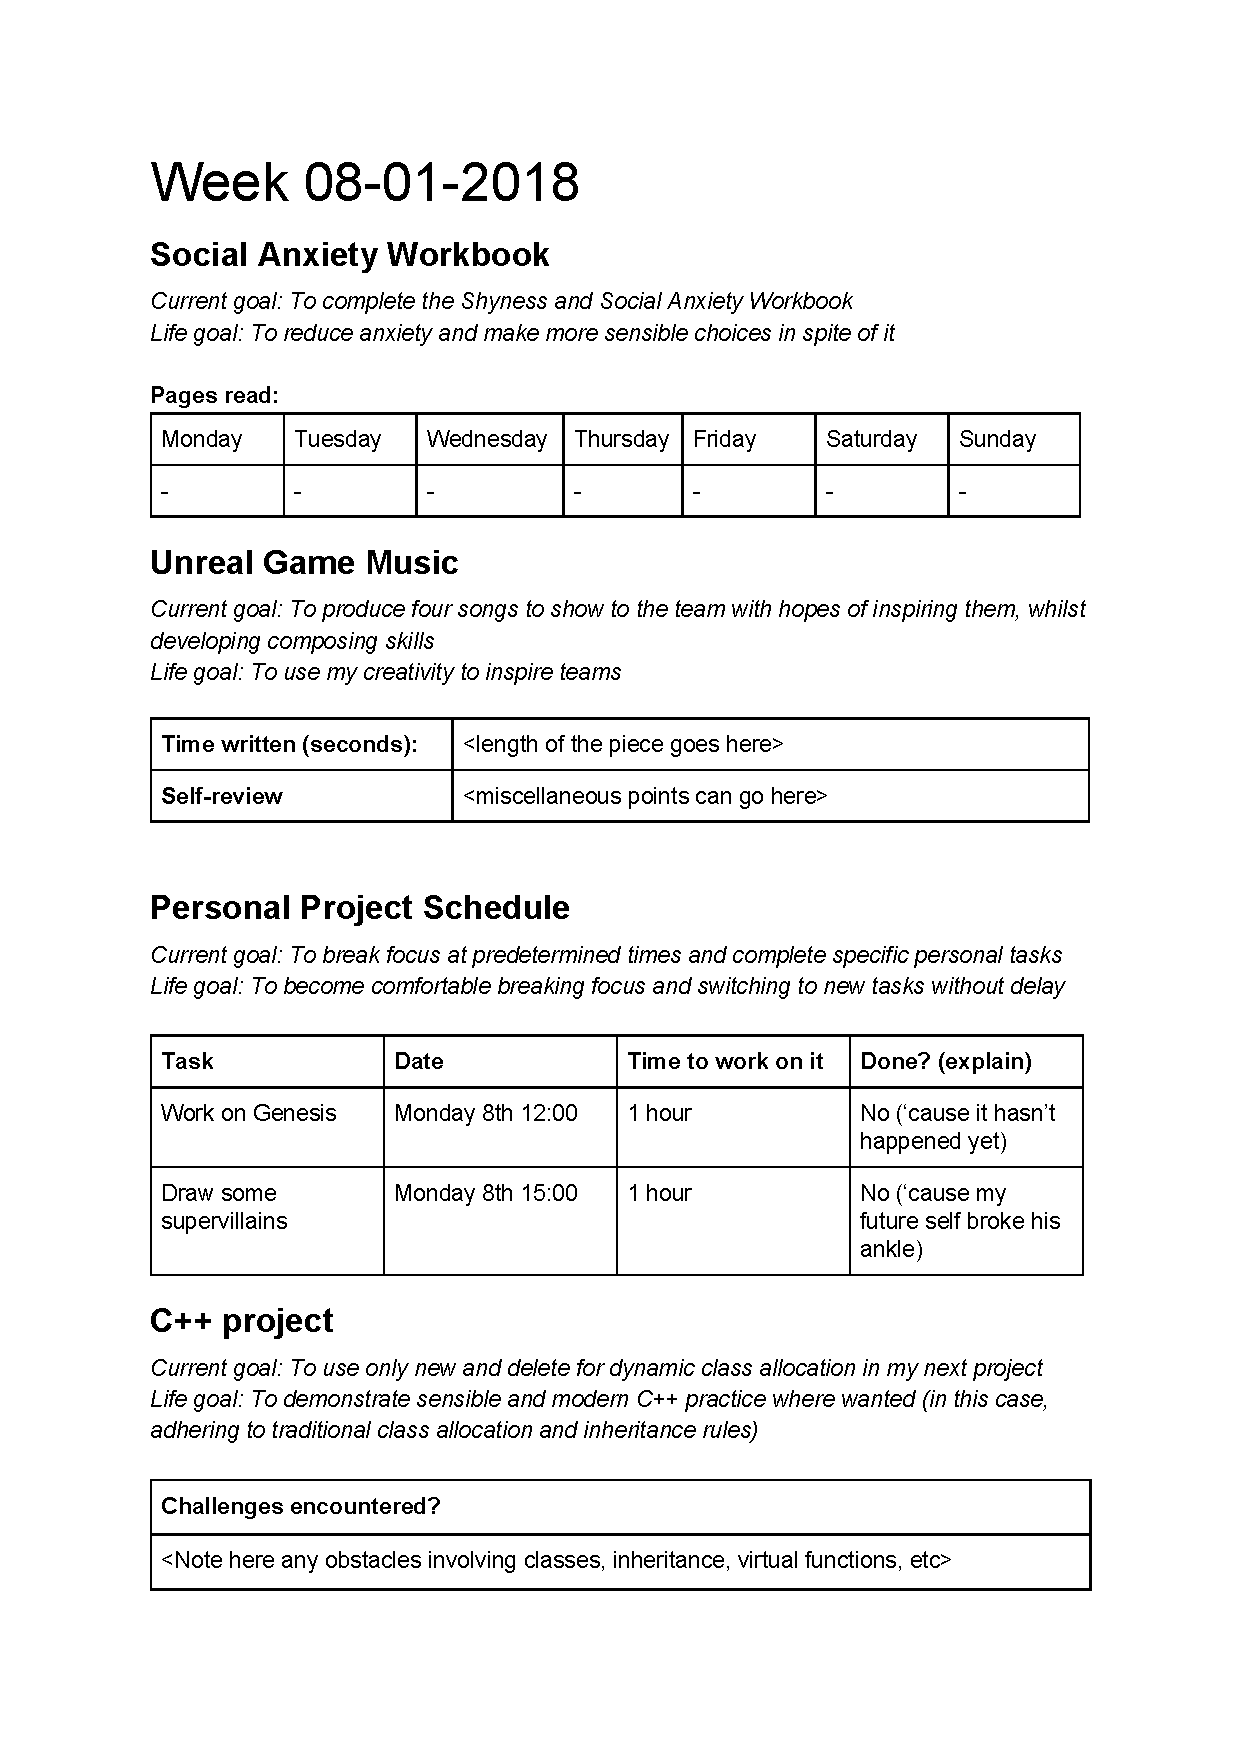
\includegraphics[width=0.7\linewidth]{diary.pdf}
	\caption{Diary template for the summer period}
\end{figure}

\end{document}
